\documentclass{report}
\usepackage{amsmath}
\usepackage{array}
\usepackage{color}
\usepackage{graphicx}
\usepackage{float} %utiliser H pour forcer a mettre l'image ou on veut
\usepackage{lscape} %utilisation du mode paysage
\usepackage{mathbbol} % permet d'avoir le vrai symbol pour les reels grace a mathbb
\usepackage{enumerate}
\usepackage{marvosym}
\usepackage{moreverb} % permet d'utiliser verbatimtab : conservation la tabulation
\usepackage{url}
\usepackage[noabbrev]{cleveref} % permet d'utiliser cref et Cref (e(E)quation(s) (..)


\setlength {\textwidth}{16cm}
\setlength {\textheight}{21cm}
\setlength {\oddsidemargin}{0cm}
\setlength{\headsep}{5pt} 

\newcommand\bn{\boldsymbol{\nabla}}
\newcommand\bo{\boldsymbol{\Omega}}
\newcommand\br{\mathbf{r}}
\newcommand\la{\left\langle}
\newcommand\ra{\right\rangle}
\newcommand\bs{\boldsymbol}
\newcommand\red{\textcolor{red}}
\newcommand\mc{\mathcal}

\renewcommand{\(}{\left(}
\renewcommand{\)}{\right)}
\renewcommand{\[}{\left[}
\renewcommand{\]}{\right]}


\begin{document}
\title{Acceleration techniques for coupled electron-photon transport}
\author{Bruno Turcksin} 
\date{}
\maketitle

\tableofcontents

\pagestyle{plain}
\pagenumbering{arabic}
\setcounter{page}{1}
\chapter{\uppercase{Introduction}}
\section{Purpose}
The transport of photons and electrons has many applications. One of them is 
radiotherapy. Radiotherapy uses photons and charged particles to 
damage the DNA of cancerous cells. When using photons, free electrons are 
generated and ionize the environment to create free radicals that damage the cells. 
The absorbed dose, defined as the energy deposited per unit of mass, is used to 
gauge whether a cell will die due to the radiation or not. Several methods can be
applied to compute the dose distribution in the body: semi-analytic,
deterministic, and Monte-Carlo methods. Monte-Carlo methods yield very
accurate results, however they are slow to converge and remain too slow for
effective clinical use \cite{acuros,comet}. Semi-analytic methods, such as
pencil-beam convolution and convolution-superposition, employ pre-calculated
Monte-Carlo dose kernels, which are then locally scaled to approximate photon
and electron transport in the presence of heterogeneities. These methods
present some issues in the presence of large density gradients such as those
found at interfaces between different materials: air, bone, lung and soft
tissue \cite{acuros,seco,krieger}. The discrete ordinates ($S_n$) method has been 
shown to be quite accurate for electron and coupled electron-photon transport 
\cite{morel_81,accuracy_1,accuracy_2}.  

One difficulty of this approach arises from the transport of electrons. Charged 
particles interact through Coulomb interactions with the  background medium. 
Such interactions predominately result in extremely small changes 
in particle direction and energy. These interactions are well characterized by the
Fokker-Planck limit of the Boltzmann equation \cite{fp_limit,morel_96}. In this limit,
the directional and energy changes are decoupled with the former modeled by the
continuous scattering operator and the latter modeled by the continuous-slowing-down 
operator. The mean-free-path and the directional change per scattering interaction 
go to zero while the momentum transfer (also called the transport-corrected 
scattering cross section) remains fixed.

When the scattering is highly forward-peaked, solving the $S_n$ transport equation 
can be challenging due to the slow convergence of standard iterative
algorithm, such as Source Iteration (SI). To speed up iterative convergence,
acceleration schemes such as Diffusion Synthetic Acceleration (DSA) and P1
Synthetic Acceleration (P1SA) are generally used for neutron transport 
\cite{dsa_ref}. These methods use a diffusion equation or the P1 equations,
and therefore, only the zeroth or the zeroth plus the first flux moment can be
accelerated. When the zeroth flux moment alone is a accelerated, these
schemes are stable (in this discussion, we ignore the possible issues due to
the possible issues due to the spatial discretization) but they are very
inefficient if the scattering is highly anisotropic. If both the zeroth and
the first flux moments are accelerated, the spectral radius of the continuous
scheme (i.e., without spatial discretization) with anisotropic scattering is
given by \cite{multisweep}:
\begin{equation}
\rho_{ani} = \max\(\rho_{iso},\frac{\mu c}{1-\mu_c}\)
\end{equation}
where $\rho_{iso}(<1)$ is the spectral radius when the scattering is
isotropic, $\mu$ $(\in [0,1])$ is the average scattering cosine, and $c$ $(\in
[0,1])$ is the scattering ratio. We see that when $\mu c > 0.5$, the scheme is
unstable. Several modifications have been proposed \cite{multisweep,russe} to
stabilize this acceleration scheme. However, for electron transport, the
scattering anisotropy is very large and some others techniques have to be
used. The angular multigrid method \cite{multigrid_1d} has proven to be very
effective to solve the $S_n$ equations with highly forward-peaked scattering
for one-dimensional slab geometry. Unfortunately, the extension of the angular
multigrid method to multidimensional geometries is unstable
\cite{multigrid_2d}. Pautz et al. added a diffusive filter to the angular
multigrid corrections as a stabilizer within the standard preconditioned
Source Iteration. This stabilized angular multigrid method converges faster
than DSA alone but the spectral radius can become arbitrary close to one for
highly anisotropic and high scattering ratio medium. In
\cite{multigrid_1d,multigrid_2d}, the authors used the traditional Source
Iteration method as solver. However, the system of linear equations can be
also be tackled using non stationary Krylov solvers, such as GMRES. A code
solving the $S_n$ equations using SI with DSA can easily be modified to use a
preconditioned Krylov solvers. In \cite{ttg}, the authors summarize the
advantageous features of GMRES as follows: ``using DSA as preconditioner for
GMRES(m) removes the consistency requirement that plagues DSA-accelerated
source iteration in multidimensional problems.'' Driven by this statement, we
will use the multidimensional angular multigrid method as a preconditioner for
GMRES in solving highly forward peaked scattering problems. Our hope is
that GMRES will be able to stabilize the proposed scheme without the use of a
filter and that the new scheme will have convergence properties similar to the
one-dimensional scheme. At the coarsest level of the angular multigrid, a DSA 
scheme or a P1SA scheme has to be used. The scheme that we will use is an 
adaptation of the Modified Interior Penalty DSA (MIP) \cite{mip}. This scheme 
was developed for discontinuous finite elements on triangular cells and it is 
symmetric and definite positive (SPD). We will adapt MIP to Bilinear
Discontinuous Finite elements (BLD) on rectangular cells and to PieceWise Linear 
Discontinuous Finite elements (PWLD) \cite{pwld_2d,pwld_3d} on arbitrary
polygonal cells. Polygonal cells can potentially reduce the number of unknowns in 
our mesh, while maintaining symmetry within the mesh. We show this potential 
reduction in number of unknowns for a hexagonal cell versus the same space divided 
using triangles:
\begin{figure}[H]
\centering
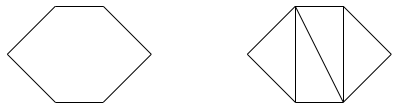
\includegraphics[width=0.5\textwidth]{./Introduction/hex_tri_cells}
\caption{Hexagonal cell versus triangle cells}
\end{figure}
We see that if there is one unknown per vertices, the hexagonal cell has 6
unknowns compared to the 12 unknowns of triangle cells. Polygonal cells can
also be used for adaptive mesh refinement (AMR) problems without having to
deal with hanging nodes \cite{arbitrary_hanging_nodes,dealII_hanging_nodes,
locally_hanging_nodes}. The left cell on the figure below is a pentagon whereas 
the two cells on the right are quadrilaterals:
\begin{figure}[H]
\centering
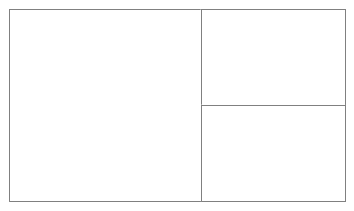
\includegraphics[width=0.3\textwidth]{./Introduction/amr}
\caption{AMR mesh}
\end{figure}
Using MIP requires us to solve SPD equations. This has usually been done using 
conjugate gradient preconditioned by SSOR, but in this research we will test the 
effectiveness of algebraic multigrid methods (AMG) to precondition the Krylov solver 
\cite{amg,amg_course}. Algebraic multigrid methods allow to use multigrid
techniques when there is no grid or that the mesh is unstructured. Instead of
using a succession of grids based on the geometry of the problems, the grids
are based on properties of the matrix. This allows to use AMG as black-box
solvers or preconditioners.

\section{Linear Boltzmann equation}
Charged particles transport can be described by the linear Boltzmann equation 
\cite{morel_81,galerkin_morel,cepxs}:
\begin{equation}
  \begin{split}
    & \bo\cdot \bn \psi(\br,\bo,E) + \Sigma_t(\br,E)\psi(\br,\bo,E) = 
    \int_0^{\infty}dE'\int_{4\pi}d\bo'\ \Sigma_s(\br,\bo'\cdot\bo,E'\rightarrow E)\\
    &\psi(\br,\bo',E')+Q(\br,\bo,E)
  \end{split}
\label{transport_p}
\end{equation}
where:
\begin{itemize}
\item $\bo = (\mu,\varphi)$ is a unit vector in the flight direction
\item $\mu = \cos(\theta)$, where $\theta$ is the directional polar angle
\item $\varphi$ is the directional azimuthal angle
\item $\mu_0 = \bo'\cdot \bo$ is the cosine of the polar angle
\item $\psi(\br,\bo,E) = vf(\br,\bo,E)$ is the angular flux
\item $v$ is the particle speed
\item $\Sigma_t(\br,E)$ is the total macroscopic cross section given by:
\begin{equation}
\Sigma_t(\br,E) = \Sigma_a(\br,E)+\Sigma_s(\br,E)
\end{equation}
\item $\Sigma_a(\br,E)$ is the absorption macroscopic cross section
\item $\Sigma_s(\br,E)$ is the scattering macroscopic cross section
\item $\Sigma_s(\br,\bo'\cdot \bo, E'\rightarrow E)$ is the differential
scattering macroscopic cross scattering
\item $Q(\br,\bo,E)$ is the volumetric source
\end{itemize}
In the rest of this work, macroscopic cross sections will be called cross
sections when no confusion is possible. Standard boundary conditions can be
applied to \cref{transport_p}. The most common is the incoming flux boundary
condition:
\begin{equation}
\psi (\br,\bo,E) = g(\br,\bo,E) \textrm{ for }\bo \cdot \bn <0 \textrm{ and }
\br \in \partial \mc{D}
\label{bc}
\end{equation}
where $\partial \mc{D}$ is the boundary of the domain. If $g=0$, \cref{bc} yields 
the vacuum boundary conditions.

\Cref{transport_p} depends on the space $(\br)$, the angle ($\bo$) and the
energy $(E)$. In this research, we are not interested in the energy variable
and therefore, we will integrate \cref{transport_p} on the energy variable. 
However, the techniques described here apply straightforwardly to the multigroup 
equations. The energy-integrated \cref{transport_p} is given by:
\begin{equation}
\bo\cdot \bn \psi(\br,\bo) + \Sigma_t(\br)\psi(\br,\bo) =
\int_{4\pi}d\bo'\ \Sigma_s(\br,\bo'\cdot\bo)\psi(\br,\bo')+Q(\br,\bo)
\label{transport_p2}
\end{equation}

The in-scattering term can be represented by Legendre polynomials $P_l$ expansion:
\begin{equation}
\begin{split}
\int_{4\pi} \Sigma_s(\br,\bo'\cdot\bo) \psi(\br,\bo') d\bo' &=
\int_{4\pi} \sum_{l=0}^{\infty} \frac{2l+1}{4\pi} \Sigma_{s,l} P_l(\bo'\cdot\bo)
\psi(\br,\bo') d\bo'\\
&= \int_{4\pi} \sum_{l=0}^{\infty} \frac{2l+1}{4\pi}\frac{4\pi}{2l+1}
\Sigma_{s,l}(\br) \times\\
&\quad \sum_{m=-l}^{l} Y_l^m(\bo)Y_l^{m,*}(\bo') \psi(\br,\bo')d\bo'\\
&= \sum_{l=0}^{\infty} \Sigma_{s,l}(\br) \sum_{m=l}^l \phi_{l,m}(\br)
Y_l^m(\bo)
\end{split}
\end{equation}
where we used:
\begin{align}
&\Sigma_s(\br,\bo\cdot\bo') = \sum_{l=0}^{\infty} \frac{2l+1}{4\pi}
\Sigma_{s,l}(\br) P_l(\bo\cdot\bo')\\
&\Sigma_{s,l}(\br) = 2\pi \int_{-1}^1 d\mu_0\ P_l(\mu_0) \Sigma_s(\br,\mu_0)\\
& P_l(\bo\cdot\bo') = \frac{4\pi}{2l+1} \sum_{m=-l}^l
Y_l^m(\bo)Y_l^{m,*}(\bo')\\
& Y_l^m(\bo) = (-1)^m \sqrt{\frac{2l+1}{4\pi} \frac{(l-m)!}{(l+m)!}} P_l^m(\mu)
e^{im\varphi}\\
&\psi(\br,\bo) = \sum_{l=0}^{\infty}\sum_{m=-l}^l \phi_{l,m}(\br) Y_l^m(\bo)
\label{ang_flux}\\
&\phi_{l,m}(\br) = \int_{4\pi} d\bo\ Y_{l}^{m,*}(\bo) \psi(\br,\bo)
\label{moments}
\end{align}
with $Y_l^m$ the spherical harmonics and $P_l^m$ the associated
Legendre polynomials. In practice, the scattering expansion is truncated 
$(\sum_{l=0}^{\infty}\rightarrow \sum_{l=0}^L)$.\\
Later, we will need the following property of the spherical harmonics:
\begin{equation}
\[\frac{\partial}{\partial\mu}(1-\mu^2)\frac{\partial}{\partial
\mu}+\(\frac{1}{1-\mu^2}\)\frac{\partial^2}{\partial \varphi}+l(l+1)\]Y_l^m(\bo)=0
\label{eigenvalue}
\end{equation}
\Cref{transport_p2} still needs to be discretized in space and angle. A
standard method to discretize the space variable is to use discontinuous
Galerkin finite elements \cite{dgfem,thick_dgfem,conv_dgfem}. The angular
discretization that we will use in this work is the $S_n$ or discrete ordinate
method developed in \cite{rad_transfer}. With this discretization, 
\cref{transport_p2} is replaced by a system of linear equations which use discrete 
angular fluxes $\(\psi(\br,\bo)\rightarrow \psi(\br,\bo_d)=\psi_d(\br)\)$ and the 
integral in \cref{moments} is replaced by a quadrature:
\begin{equation}
\phi_{l,m}(\br) = \sum_d w_d Y_{l}^{m,*}(\bo_d) \psi_d(\br)
\label{moments_2}
\end{equation}
where $w_d$ are the weights associated to the quadrature. Therefore, the $S_n$
discretization of \cref{transport_p2} is given by:
\begin{equation}
\bo_d\cdot\bn \psi_d(\br) + \Sigma_t(\br)\psi_d(\br) = \sum_{l=0}^L
\Sigma_{s,l}(\br) \sum_{m=-l}^l \phi_{l,m} Y_l^m(\bo_d) + Q_d(\br)
\label{transport_sn}
\end{equation}
\Cref{transport_sn} can be written in a more compact way:
\begin{equation}
L\Psi = M\Sigma D\Psi + Q
\label{transport_operator}
\end{equation}
where:
\begin{itemize}
\item $L$ is the streaming operator $\bo_d \cdot \bn \bullet + \Sigma_t(\br)
\bullet$
\item $M$ is the moments-to-directions operator $\Psi = M\Phi$
\item $D$ is the directions-to-moments operator $\Phi = D\Psi$
\item $\Sigma$ is the scattering cross-section operator
\end{itemize}


\section{Organization of the Dissertation}
The dissertation is organized as follows.\\

\noindent In Chapter II, we introduce the Boltzmann-Fokker-Planck (BFP)
equation used to describe the transport of charged particles. In the BFP equation
the Fokker-Planck operator is added in the Boltzmann equation in order to simplify
the treatment of the highly forward-peaked scattering kernel. We show that the
Fokker-Planck equation is an asymptotic limit of the Boltzmann equation when the
mean free path goes to zero and $\mu_0$ goes to one. The Fokker-Planck
equation is not valid for every forward-peaked scattering kernel and
therefore, the BFP has limitations. In particular, the Henyey-Greenstein kernel
and the Rutherford cross section do not satisfy the Fokker-Planck equation.
Being aware of these limitations, we introduce the Fokker-Planck cross
section, which allows to reduce the Fokker-Planck equation and the BFP equation
to a Boltzmann equation. Fokker-Planck cross sections cannot be used with any
quadrature, special quadratures known as Galerkin quadratures must be adopted.
The importance and the properties of these quadratures are explained in
details at the end of Chapter II.\\

\noindent In Chapter III, we introduce the angular multigrid methods for 
transport with highly forward-peaked scattering. We recall the previous works 
on the topic and we discuss the problems encountered for multidimensional 
problems. The original angular multigrid method for one-dimensional geometry
shown very quick convergence for problems with highly forward-peaked
scattering whereas DSA is ineffective. Unfortunately, the generalization to
multidimensional geometry required a filter to stabilized the methods which
was not as efficient as in one dimensional geometry. When the scattering
becomes very anisotropic, the angular multigrid method become ineffective. In
that Chapter, we show that if the angular multigrid method is recast as a
preconditioner for a Krylov solver, the method does not need to be stabilized
and is always effective and efficient.\\

\noindent In Chapter IV, we discuss the spatial discretizations: BiLinear
Discontinuous finite elements (BLD) and PieceWise Linear Discontinuous finite
elements (PWLD). The BLD finite elements are used on rectangular cells while
the PWLD finite elements can be used on any polygonal cells. In that Chapter, 
we adapt the Modified Interior Penalty DSA developed for triangular cells to
rectangular and polygonal cells. This DSA discretization is used as the
coarsest level of the angular multigrid method developed in Chapter III. In
Chapter IV, we also investigate algebraic multigrid methods as preconditioners
to solve MIP. Since MIP is symmetric and definite positive (SPD), the most
common method to solve it, is to use conjugate gradient (CG) preconditioned by
SSOR. It is not the only method and we show that CG preconditioned by
algebraic multigrid methods is superior if the matrix associated to MIP can be
stored.\\

\noindent In Chapter V, we finish with some concluding remarks and suggestions for
future developments.

\section{Transport equation}
Inelastic interactions, collisional and radiative scattering, can be divided
into two classes : ``catastrophic" interactions that result in large-energy
losses and ``soft" interactions that result in small-energy losses. p25 CEPXS

\section{Fokker-Planck cross section}
In this section, we derive the Fokker-Planck scattering cross section such
that the Fokker-Planck operator can be approximated by the Boltzmann operator.  
First we recall the BFP equation \cref{bfp}:
\begin{equation}
\begin{split}
&\bo\cdot\psi+(\Sigma_{s,reg}+\Sigma_a)\psi=\sum_{l=0}^{\infty}\sum_{m=-l}^l
Y_l^m(\bo)\int_E^{E/\alpha}\Sigma_{s,l,reg}(E'\rightarrow
E)\phi_{l,m}(E')dE'+\\
&\frac{\partial(S\psi)}{\partial E}+\frac{\alpha}{2}\(\frac{\partial}{\partial
\mu}(1-\mu^2) \frac{\partial}{\partial
\mu}+\frac{1}{(1-\mu^2)}\frac{\partial^2}{\partial\varphi^2}\)\psi+Q,
\end{split}
\end{equation}
where we used $\alpha = 2T$.
Let us define:
\begin{align}
\mc{L}_{FP}^{\alpha} \psi &= \frac{\alpha}{2} \frac{\partial}{\partial \mu}
(1-\mu^2) \frac{\partial}{\partial \mu}\psi \label{gamma_alpha}\\
\mc{L}_{FP}^e\psi &=\frac{\partial}{\partial E}S\psi +
\frac{1}{2}\frac{\partial^2}{\partial E^2} R \psi. \label{gamma_e}
\end{align}
We note that $\mc{L}_{FP}^{\alpha}$ causes particles to redistribute in
direction without energy change, while $\mc{L}_ {FP}^e$ causes particles to
redistribute particles in energy without directional change. Therefore,
$\mc{L}_{FP}^{\alpha}$ can be approximated using the following cross section:
\begin{equation}
\Sigma_s(\mu_0,E'\rightarrow E) = \Sigma_s^{\alpha}(\mu_0,E) \delta(E'-E),
\end{equation}
where $\Sigma_{s}^{\alpha} (\mu_0,E) = \frac{\alpha(E)}{1-\mu_s} \frac{1}{2\pi}
\delta(\mu_0-\mu_s)$ and $\mu_s$ is a parameter; while $\mc{L}_{FP}^e$ 
should be approximated by a cross section of the form:
\begin{equation}
\Sigma_s(\mu_0,E'\rightarrow E) = \Sigma_s^e(E'\rightarrow E) \frac{1}{2\pi}
\delta(\mu_0-1).
\end{equation}

\subsection{Legendre polynomial expansion of $\Sigma_s^{\alpha}$}
Next, we express the Legendre polynomial expansion of
$\Sigma_s^{\alpha}(\mu_0)$ ($E$ was dropped for brevity) 
as it has been done in \cite{morel_89,morel_81,morel_96}. We will focus on
$\mc{L}_{FP}^{\alpha}$ since this research we solve the energy-integrated
Boltzmann equation and, therefore, the $\mc{L}_{FP}^e$ operator does not appear in
the equation that we solve. Because $\Sigma_s^{\alpha}$ does not change 
particle energy, it corresponds to a within-group cross section. We define:
\begin{align}
  \mc{L}_B^{\alpha} &= \Sigma_s^{\alpha} \mc{L}_B\\
  \mc{L}_{FP}^{\alpha} &= \frac{\alpha}{2}\mc{L}_{FP},
\end{align}
and thus:
\begin{align}
\mc{L}_B^{\alpha}Y_l^m(\bo) &= (\Sigma_{s,l}^{\alpha}-\Sigma_{s,0}^{\alpha})
Y_l^m(\bo) \label{gamma_b_alpha_p}\\
\mc{L}_{FP}^{\alpha} Y_l^m(\bo) &= -\frac{\alpha}{2} l(l+1) Y_l^m(\bo).
\label{gamma_fp_alpha_p}
\end{align}
Using \cref{ang_flux,gamma_b_alpha_p,gamma_fp_alpha_p}, we can define 
$\Sigma_s^{\alpha}$ such that:
\begin{equation}
\mc{L}_B^{\alpha}\psi=\mc{L}_{FP}^{\alpha}\psi,
\end{equation}
by setting:
\begin{equation}
\Sigma_{s,l}^{\alpha}-\Sigma_{s,0}^{\alpha} = -\frac{\alpha}{2}l(l+1),
\label{sigma_m_sigma}
\end{equation}
with $l=1,\hdots,L$. Choosing $\Sigma_{s,L}^{\alpha}=0$ to minimize 
$\Sigma_{s,0}^{\alpha}$ and \cref{sigma_m_sigma} becomes:
\begin{equation}
\Sigma_{s,l}^{\alpha} = \frac{\alpha}{2}\(L(L+1)-l(l+1)\),\ \  l=0,\hdots,L.
\label{eq_297}
\end{equation}
Using appropriate quadrature sets and expansion orders, the $S_n$
representation of $\mc{L}_{FP}^{\alpha}$ is equivalent to the one obtained by
interpolating the discrete angular flux values with a polynomial.

Next, we look at the behavior of $\Sigma_s^{\alpha}$ when the degree of the expansion 
is increased. First, we should note that the momentum transfer of
$\Sigma_s^{\alpha}$ is exact for any expansion order:
\begin{equation}
\begin{split}
2\pi \int_{-1}^1 \Sigma_s^{\alpha}(\mu_0) (1-\mu_0) d\mu_0 &=
\Sigma_{s,0}-\Sigma_{s,1}\\
&=\frac{\alpha}{2} L(L+1) - \frac{\alpha}{2} (L(L+1)-2)\\
&=\alpha.
\end{split}
\end{equation}
With \cref{eq_297}, the average cosine of the scattering angle
becomes:
\begin{equation}
\begin{split}
\bar{\mu}_0 &= \frac{\Sigma_{s,1}^{\alpha}}{\Sigma_{s,0}^{\alpha}}\\
&=\frac{L(L+1)-2}{L(L+1)}.
\end{split}
\end{equation}
It is easily seen that when $L$ increases, $\bar{\mu}_0$ goes to one and
$\Sigma_s^{\alpha}$ becomes increasingly forward-peaked. The
total magnitude of $\Sigma_s^{\alpha}(\mu_0)$ becomes unlimited when $L$ goes to
$\infty$:
\begin{equation}
\Sigma_{s,0}^{\alpha} = \frac{\alpha}{2} L (L+1).
\end{equation}
This shows that $\mc{L}_{FP}^{\alpha}$ corresponds to a continuous-deflection 
interaction. The particles are continuously 
deflected with the mean deflection per unit pathlength given by the momentum transfer.

$\mc{L}_{B}^{\alpha}$ converges to $\mc{L}_{FP}^{\alpha}$ when $\mu_s$ tends
to one but it does not converge uniformly. For any fixed value of $\mu_s$, 
the high-order eigenvalues of $\mc{L}_{FP}^{\alpha}$ are grossly underestimated 
by $\mc{L}_B^{\alpha}$. Fortunately, this is error in the high-order eigenvalues 
is usually unimportant \cite{morel_96}.

\section{Galerkin quadratures}
Until now, we have not described which angular quadrature should be used to
correctly treat high orders of anisotropy. We have only
stated that we need an appropriate quadrature but we did not explain what we
required. In this section, we introduce the Galerkin quadrature. Morel
first introduced them in \cite{galerkin_morel}; here, we
will introduce them following the presentation made in \cite{pautz_fp}. 

First, we start by recalling the definition of $\psi$ and $\phi_{l,m}$:
\begin{equation}
  \begin{split}
    \phi_{l,m}(\br) &= \int_{4\pi} d\bo' \psi(\br,\bo') Y_l^{m,*}\\
                    &=(\bs{D} \Psi)_{l,m}
  \end{split}
  \label{D2M}
\end{equation}
where $\bs{D}$ is the direction-to-moment operator. We also have:
\begin{equation}
  \begin{split}
    \Psi(\br,\bo) &= \sum_{l=0}^{\infty} \sum_{m=-l}^l Y_l^m(\bo)\phi_{l,m}(\br)\\
                  &= \bs{M}\Phi(\br)
  \end{split}
  \label{M2D}
\end{equation}
where $\bs{M}$ is the moment-to-direction operator. By combining \cref{D2M,M2D}, 
we obtain:
\begin{equation}
  (\bs{I}-\bs{MD})\Psi = 0
  \label{identity_alpha}
\end{equation}
since for analytic transport $\bs{M}=\bs{D}^{-1}$. $\bs{I}$ is the identity operator.

Now, we define \cite{pautz_fp}:
\begin{align}
\epsilon &= 1 - \la \bar{\mu}_0\ra \label{eps_pautz} \\
    \gamma &= \la\overline{(1-\mu_0)^2}\ra \label{gamma_pautz}\\
    A(\br) &= \frac{1-\bar{\mu}_0(\br)}{\epsilon}\label{A_pautz}\\
  \Sigma_a &= \hat{\Sigma}_a \label{hat_sig_a_0}\\
\Sigma_{s,l} &= \frac{\hat{\Sigma}_{s,l}(\br)}{\epsilon} \label{hat_sig_a_1}\\
\Sigma_{s,l}(\br) &=\Sigma_{s,0}(\br) \(1-\frac{l(l+1)}{2}A(\br)\epsilon +
  O(\gamma)\) \label{hat_sig_a_2}
\end{align}
where $\la X \ra$ is a typical value of $X$. Using \crefrange{eps_pautz}{hat_sig_a_2} 
in \cref{transport_sn}, we get:
\begin{equation}
\begin{split}
&\bo_k\cdot\bn\psi_k(\br) + \(\Sigma_a(\br)+\Sigma_{s,0}(\br)\) \psi_k(\br)
=\\
& \sum_{l=0}^{N-1} \sum_{m=-l}^l Y_l^m(\bo_k) \phi_{l,m}(\br)
\frac{\hat{\Sigma}_{s,0}(\br)}{\epsilon}\(1-\frac{l(l+1)}{2}A(\br)\epsilon +
O(\gamma)\) + Q(\br,\bo_k)
\end{split}
\label{discr_eps}
\end{equation}
where:
\begin{align}
\psi_k(\br) &= \psi(\br,\bo_k)\\
\phi_{l,m}(\br) &= \sum_{k=1}^K w_k Y_l^{m,*}(\bo_k) \psi_k(\br). \label{phi_p}
\end{align}
$w_k$ and $\bo_k$ are the quadrature weights and directions of a 
quadrature set of order $N$. For triangular quadrature sets, $K=N$ in 1D, 
$K=\frac{N(N+2)}{2}$ in 2D and $K=N(N+2)$ in 3D. \Cref{discr_eps} yields:
\begin{equation}
\begin{split}
&\bo_k\cdot\bn \psi_k(\br) +\hat{\Sigma}_a(\br)\psi_k(\br)+
\frac{\hat{\Sigma}_{s,0}(\br)}{\epsilon} \(\psi_k(\br)-\sum_{l=0}^{N-1}
\sum_{m=-l}^m  Y_l^m(\bo_k) \phi_{l,m}\)\\
&=-\frac{\(\Sigma_{tr}(\br)-\hat{\Sigma}_a(\br)\)}{2} \sum_{l=0}^{N-1}
\sum_{m=-l}^{l} l(l+1) Y_l^m(\bo_k) \phi_l^m(\br)+
 Q(\br,\bo_k) + O\(\frac{\gamma}{\epsilon}\).
\end{split}
\label{discr_eps_manip}
\end{equation}
We insert the asymptotic ansatz:
\begin{align}
\psi &= \psi^{(0)} + \epsilon \psi^{(1)} + \epsilon^2\psi^{(2)}+\hdots\\
\phi_{l,m} &= \phi_{l,m}^{(0)} + \epsilon \phi_{l,m}^{(1)} + \epsilon^2
\phi_{l,m}^{(2)}+\hdots
\end{align}
into \cref{discr_eps}. The terms of $O(1)$ give:
\begin{equation}
\begin{split}
\phi_{l,m}^{(0)}(\br) &= \sum_{k=1}^K w_k Y_l^{m,*}(\bo_k) \psi_k^{(0)}(\br)\\ 
                      &= (\bs{D}_N\Psi^{(0)})_{l,m}.
\end{split}
\label{D2M_disc}
\end{equation}
Now we insert the ansatz into \cref{discr_eps_manip} and we look at the terms
of $O(\epsilon^{-1})$:
\begin{equation}
\begin{split}
\psi_d^{(0)}(\br) &=\sum_{l=0}^{N-1} \sum_{m=-l}^l Y_l^m(\bo_k) 
\phi_{l,m}^{(0)}(\br)\\
&= (\bs{M}_N\Phi^{(0)})_d
\end{split}
\label{M2D_disc}
\end{equation}
there is no $O(\gamma)$ term, since $\gamma\rightarrow 0$ when 
$\epsilon\rightarrow 0$, i.e., that there are no
$O(1)$ components in $\gamma$. \Cref{D2M_disc,M2D_disc} may be combined to give:
\begin{align}
  &(\bs{I}-\bs{M}_N\bs{D}_N)\Psi^{(0)} = 0 \label{identity_a}\\
  &(\bs{I}-\bs{D}_N\bs{M}_N)\Phi^{(0)} = 0 \label{identity_b}.
\end{align}
This means that $\Psi^{(0)}$, respectively $\Phi^{(0)}$, must be in the kernel
of $\bs{I}-\bs{M}_N \bs{D}_N$, respectively $\bs{I}-\bs{D}_N \bs{M}_N$. Using 
\cref{phi_p}, \cref{identity_b} becomes successively:
\begin{equation}
  \(\bs{I}-\bs{D}_N \bs{M}_N\) \bs{D}_N \Psi^{(0)} = 0
\end{equation}
\begin{equation}
  \(\bs{D}_N-\bs{D}_N \bs{M}_N \bs{D}_N\) \Psi^{(0)} = 0
\end{equation}
\begin{equation}
  \bs{D}_N(\bs{I}-\bs{M}_N \bs{D}_N)\Psi^{(0)} = 0,
\end{equation}
which is always satisfied if \cref{identity_a} is satisfied.
Therefore, if \cref{identity_a} is satisfied, \cref{D2M_disc,M2D_disc} are
automatically satisfied.

A sufficient condition to satisfy \cref{identity_a} is that $\bs{M}_N \bs{D}_N
=\bs{I}$. This is of course true if $\bs{D}_N=\bs{M}_N^{-1}$ like in analytic 
transport. Obviously for $\bs{M}_N$ and $\bs{D}_N$ to be inverse of each other, 
the matrices have to be square. Thus, the number of moments in the scattering 
expansion must be equal to number of discrete angles. In one-dimension,
$\bs{D}_N = \bs{M}_N^{-1}$ is satisfied if the 
quadrature set integrates exactly any polynomials of degree $2N-1$, like the 
Gauss-Legendre quadrature does. In multidimensional problems, the standard 
quadrature sets use more discrete angles than there are scattering moments. 
Therefore, $\bs{M}_N$ and $\bs{D}_N$ are rectangular matrices and they cannot 
be inverse of each other. In this case, \cref{identity_a} can only be satisfied if 
$\Psi^{(0)}$ is in the kernel of $(\bs{I}-\bs{M}_N\bs{D}_N)$. This can be achieved 
only if $\Psi^{(0)}$ satisfies nonphysical constraints \cite{pautz_fp}. If 
\cref{identity_a} is not satisfied, the asymptotic ansatz is not valid and 
there is no $O(1)$ solution to \cref{discr_eps,phi_p}.\\
If we assume that $\bs{M}_N \bs{D}_N=\bs{I}$, then the $O(\epsilon)$ terms in 
\cref{phi_p} give:
\begin{equation}
  \begin{split}
    \phi_{l,m}^{(1)}(\br) &= \sum_{k=1}^K w_k Y_{l}^{m,*} (\bo_k) \psi_k^{(1)}(\br)\\
                          &=(\bs{D}_N\Psi^{(1)})_{l,m}
  \end{split}
\end{equation}
In \cref{discr_eps_manip}, the $O(1)$ terms give:
\begin{equation}
  \begin{split}
    &\bo_k\cdot \bn \psi_k^{(0)}(\br) + \hat{\Sigma}_a(\br)\psi_k^{(0)}(\br) +
    \hat{\Sigma}_{s,0}(\br) \(\psi_k^{(1)} (\br) - \sum_{n=0}^{N-1}
    \sum_{m=-l}^{l} Y_l^m (\bo_k)\phi_{l,m}^{(1)}(\br)\)\\
    &=-\frac{\Sigma_{tr}(\br)-\hat{\Sigma}_a(\br)}{2} \sum_{l=0}^{N-1}
    \sum_{m=-l}^l  l(l+1) Y_l^m(\bo_k)
    \phi_{l,m}^{(0)}(\br)+ Q(\br,\bo_k) + O\(\frac{\gamma}{\epsilon}\).
  \end{split}
  \label{O_1_terms}
\end{equation}
Now, we want the scattering term on the left side of \cref{O_1_terms} to
disappear in order to keep only $\psi_k^{(0)}$ and $\phi_{l,m}^{(0)}$. This 
is possible only if:
\begin{equation}
\psi_d^{(1),*}(\br) = \psi_d^{(1)}(\br)
\label{psi_1_star_old}
\end{equation}
where:
\begin{equation}
  \begin{split}
    \psi_d^{(1),*} &= \sum_{l=0}^{N-1}\sum_{m=-l}^l Y_l^m(\bo_k) 
    \phi_{l,m}^{(1)}(\br)\\
                   &= (\bs{M}_N\Phi^{(1)})_d\\
                   &=(\bs{M}_N \bs{D}_N \Psi^{(1)})_d
  \end{split}
  \label{psi_1_star}
\end{equation}   
which is satisfied because of our previous assumption that $\bs{M}_N \bs{D}_N
= \bs{I}$. \Cref{O_1_terms} yields:
\begin{equation}
\begin{split}
  &\bo_k \cdot \bn \psi_k^{(0)}(\br)+\hat{\Sigma}_a(\br) \psi_k^{(0)}(\br) =
  \frac{\Sigma_{tr}(\br)-\hat{\Sigma}_a(\br)}{2}
  \(\(\frac{\partial}{\partial \mu}(1-\mu^2)\frac{\partial}{\partial
  \mu}+\right. \right.\\
  &\left.\left. \(\frac{1}{1-\mu^2}\)\frac{\partial^2}{\partial \varphi^2}\)
  \tilde{\psi}^{(0)} (\br,\bo)\)_{\bo=\bo_k}+ Q(\br,\bo_k) + 
  O\(\frac{\gamma}{\epsilon}\)
\end{split}
\label{last_pautz}
\end{equation}
where $k=1,\hdots,K$ and $\tilde{\psi}^{(0)}(\br,\bo)$ is an interpolant
through the points $P_k=\{\bo_k,\psi_k^{(0)}(\br,\bo)\}$. ``In one-dimensional 
geometry, $\tilde{\psi}^{(0)}(\br,\bo)$ is the $(N-1)-$order
polynomial interpolant through the points $P_k$. In multidimensional
geometries, $\tilde{\psi}^{(0)}(\br,\bo)$ is the spherical harmonic
interpolant through the points $P_k$'' \cite{pautz_fp}. A quadrature which 
satisfies the relation $\bs{D}_N = \bs{M}_N^{-1}$ is called a ``Galerkin'' quadrature 
because Morel derived it by using a Galerkin weighting method \cite{galerkin_morel}.

In \cite{galerkin_morel}, Morel made the following suggestions to find the 
correct limit using the $S_N$:
\begin{description}
\item [One-dimensional geometry:] The Gauss-Legendre quadrature set is the
  only quadrature set which is a Galerkin quadrature.
\item [Multidimensional geometry:] The standard quadrature sets have fewer 
  moments than discrete angles. Therefore to satisfy $\bs{D}=\bs{M}^{-1}$, spherical
  harmonics of higher order need to be added to increase the number of moments
  up to the number of angular flux. Morel in \cite{galerkin_morel} and Reed in 
  \cite{reed} proposed an heuristic algorithm to choose the spherical 
  harmonics for multidimensional geometries. If we use the real spherical
  harmonics defined by:
  \begin{equation}
    Y_{l,m}^c = \left\{
      \begin{aligned}
        &Y_l^0 & \textrm{ if } m=0\\
        &\frac{1}{\sqrt{2}} \(Y_l^m+(-1)^{m} Y_l^{-m}\) & \textrm{ if } m> 0
      \end{aligned}
      \right.
  \end{equation}
  \begin{equation}
    Y_{l,m}^s = \frac{1}{i\sqrt{2}}(Y_l^{-m}-(-1)^{m}Y_l^m) \textrm{ if } m<0
  \end{equation}
  and a two-dimensional triangular quadrature set, the selection rules to build 
  $\bs{M}$ are the following:
  \begin{itemize}
    \item Take $Y_{l,m}^c$ if $l\in[0,N-1]$, $m\in[0,l]$, and $l+m$ is even.
    \item Take $Y_{l,m}^s$ if ($l \in [1,N-1]$, $m\in[1,l]$, and $l+m$ is
      even) or if ($l=N$, $m\in[1,l]$, and $l+m$ is even).
  \end{itemize}
  For three dimensional triangular quadrature sets, the spherical harmonics
  are:
  \begin{itemize}
    \item Take $Y_{l,m}^c$ if ($l \in [0,N-1]$ and $m\in[0,l]$) or if ($l =
      N$, $m\in[1,N-1]$, and $m$ is odd).
    \item Take $Y_{l,m}^s$ if ($l\in [1,N]$ and $m\in[1,l]$) or if ($l=N+1$,
      $m\in[2,N]$ and $m$ is even).
  \end{itemize}
\end{description}
General necessary conditions and explanations of the heuristic rules above
have been analyzed in \cite{galerkin_sanchez}.

Using a standard $S_n$ quadrature may led to an unphysical solution for
charged particle transport. To further demonstrate the importance of Galerkin
quadrature, we define the scattering ratio matrix $\bs{C}$ by:
\begin{equation}
\bs{C} = \frac{1}{\Sigma_t}\bs{D}\bs{M}\bs{\Sigma},
\end{equation}
where $\bs{\Sigma}$ is the scattering matrix containing the moments of the
scattering cross sections on its diagonal.
$\bs{C}$ is a diagonal matrix whose entries are the scattering ratios
$c_l=\frac{\Sigma_{s,l}}{\Sigma_t} \leq 1$. The fact that $\bs{MD}=\bs{I}$
assures a one-to-one relation between the angular flux and the flux moments;
furthermore, the orthogonality of all spherical harmonic functions used in the
angular flux representation is preserved. However, if a standard quadrature is
employed, then $\bs{D} = \bs{M}^T \bs{W}$, where $\bs{W}$ is the diagonal
matrix of weights, and inexact integration occurs for the set of spherical
harmonics than span $\bs{M}$. Thus, $\bs{C}$ will differ from
$\frac{\bs{\Sigma}}{\Sigma_t}$ and its eigenvalue could exceed unity. This is
equivalent to numerically adding multiplication into the medium and, depending
on the amount of leakage present in the geometrical configuration, the
steady-state transport equation may not reach a steady state solution
\cite{pautz_fp}.

A very important property of the Galerkin quadratures is that they treat the
delta function scattering exactly. This is very important for two reasons. 
The first reason is that in charged-particle transport, some cross sections 
have the following form:
\begin{equation}
\Sigma^{k\rightarrow g}(\mu_0) = \Sigma^{k\rightarrow g} \delta(\mu_0-1),
\end{equation}
where $\Sigma^{k\rightarrow g}(\mu_0)$ is the differential cross section
associated with a transfer from group $k$ to group $g$. Thus, it is essential
that delta function scattering be treated exactly. The second reason, which is
more important for us since we work with energy-integrated equation, is that for 
electron scattering, the extended transport correction \cite{lathrop} can be 
used to reduce the within-group scattering cross sections by two orders of 
magnitude or more \cite{morel_79}. Without the extended transport correction, 
the high order of the flux moments are very important and DSA does not 
accelerate the convergence of the solver. Because the Galerkin method treats 
delta function  scattering exactly, the extended transport correction does not
modify the solution of the problem \cite{morel_79}. This is very interesting 
since it allows to reduce significantly the higher moments of the scattering
cross-section expansion without losing of accuracy. Showing this property is
quite simple given what we have presented thus far. We know that in the analytic case
we have:
\begin{equation}
\int_{4\pi} \delta(\mu_0-1) \psi(\bo')\ d\bo' = \psi(\bo).
\end{equation}
When the scattering source is discretized, we have $\bs{\Sigma}=\bs{I}$.
Therefore, it is obvious that:
\begin{equation}
  \bs{D\Sigma M}\Psi = \Psi.
\end{equation}

To really understand the Galerkin quadrature, it is interesting to recall 
the development made in \cite{galerkin_morel}. First, we expand the
one-dimensional angular flux on an interpolatory trial space:
\begin{equation}
\Psi(\mu) = \sum_{d=1}^N \psi_d B_d(\mu).
\label{psi_b}
\end{equation}
Methods for generating the interpolatory basis function can be found in 
\cite{galerkin_morel}. Next, we expand the scattering source on the Legendre
polynomials:
\begin{equation}
\mc{S}(\mu) = \sum_{l=0}^{\infty} \frac{2l+1}{2} \xi_l P_l(\mu)
\label{S_mu_2}
\end{equation}
where:
\begin{equation}
  \xi_l = \int_{-1}^1 \mc{S}(\mu) P_l(\mu) d\mu.
\end{equation}
Now, we use the interpolatory trial space to approximate $S(\mu)$:
\begin{equation}
\tilde{\mc{S}}(\mu) = \sum_{d=1}^N \tilde{\mc{S}}_d B_d(\mu)
\label{tilde_s_mu}
\end{equation}
Since a Galerkin method is used, the residual associated with the trial space 
approximation must be orthogonal to the weighting
space. The residual associated with \cref{tilde_s_mu} is given by:
\begin{equation}
Res(\mu) = \tilde{\mc{S}}(\mu) - \mc{S}(\mu).
\label{R_mu}
\end{equation}
Since the Legendre polynomials form a basis the weighting space, we
orthogonalize against the Legendre polynomials:
\begin{equation}
\int_{-1}^1 Res(\mu) P_l(\mu) d\mu = 0.0,\ \ l=0,\hdots,N-1.
\label{int_r_mu}
\end{equation}
\Cref{int_r_mu} is satisfied if:
\begin{align}
&\tilde{\xi}_l = \xi_l,\ \ l=0,\hdots,N-1 \label{xi_vs_xi}\\
&\tilde{\xi}_l = \int_{-1}^1 \tilde{\mc{S}}(\mu) P_l(\mu) d\mu.
\end{align}
The main idea of the Galerkin quadrature can be seen on \cref{xi_vs_xi}: ``the
discrete scattering source values are chosen such that the interpolatory
representation for that scattering source has the same Legendre moments
through degree $N-1$ as the exact scattering source calculated with the
interpolatory representation for the angular flux \cite{galerkin_morel}''. 
Because all the elements of the weighting space can be expressed as a linear
combination of Legendre polynomials $P_l$ with $l<N$ and $\int_{-1}^{1}
P_l(x)P_m(x)\ dx=0$ for $l\neq m$, only the first $N-1$ cross-section moments
are needed.

Now, we compare the cross-section expansion for the Galerkin method and
the $S_n$ method. Both the Galerkin method and the standard $S_n$ method use
the Legendre expansion of the cross section. However, whereas the $S_n$ method
actually uses the Legendre expansion, the Galerkin scattering source is
fully consistent with the exact cross section. It is not
important whether or not the Legendre cross-section expansion represent
accurately the scattering cross section. What is important is that
$\tilde{S}(\mu)$ is an accurate approximation of $S(\mu)$. This is a crucial 
property for charged particle transport. For example, the delta
function expansion of finite degree is never converged, and this is an issue if a 
$S_n$ method with a standard quadrature is used. However, as proved earlier, 
the scattering source computed by the Galerkin method is treated exactly.

If the scattering is isotropic, the $S_n$ method appears superior to the
Galerkin, since the Galerkin requires the number of flux moments to be equal
to the number of angular flux. Fortunately, if the higher order cross-sections
moments are zero, only the first rows of $\bs{D}$ and the first columns of
$\bs{M}$ need to be kept.

A Galerkin quadrature set and its companion quadrature sets (standard
quadrature sets associated to the Galerkin quadrature set) are different only
if the expansion order of the scattering cross section is high enough. When the 
scattering is isotropic, the Galerkin quadrature set is the same than its
companion set. Even when the scattering is highly anisotropic, the results
given by the Galerkin set and its companion set can be very close. This is due
to the fact the high order moments of the scattering cross section are often,
but not always, very small.


% bibliography
\bibliographystyle{unsrt}
\bibliography{biblio}
% include all the references
%\nocite{*}

\end{document}

